Познакомимся с библиотекой SFML на простых практических примерах. Для этого нужно скачать бибилотеку на компьютер с официального сайта: \url{https://www.sfml-dev.org/download/}, затем понадобиться провести подключение всех компонентов библиотеки в рабочую область.

Рассмотрим простейшие функции, которые помогут написать первую тестовую программу (вывод простых фигур на экран). Для начала понадобится подключить заголовочный файл, позволяющий работать непосредственно с графикой:

\begin{lstlisting}[style=myStyle, numbers=none]
#include <SFML/Graphics.hpp>
\end{lstlisting}

После подключения появляется возможность использовать новые функции. В \texttt{main} инициализируем новое окно размером 800 на 600 пикселей следующим образом:

\begin{lstlisting}[style=myStyle, numbers=none]
sf::RenderWindow window(sf::VideoMode(800, 600), "Shapes");
\end{lstlisting}

Теперь определимся с формой, размером, цветом и позицией отображаемых фигур и инициализируем их, задав нужные параметры с помощью простых и интуитивно понятных методов:

\begin{lstlisting}[style=myStyle]
sf::CircleShape circle(50.f);
circle.setFillColor(sf::Color::Red);
circle.setPosition(100.f, 100.f);

sf::RectangleShape rect(sf::Vector2f(120.f, 60.f));
rect.setFillColor(sf::Color::Blue);
rect.setPosition(300.f, 200.f);
\end{lstlisting}

После инициализации всех необходимых элементов можно приступить к созданию \textbf{основного цикла}, который реализует всю логику программы и обеспечивает её работу. Он включает в себя такие этапы как: обработка событий, обновление логики, отрисовка. В нашей программе отсутствует логика, поэтому мы пропускаем второй этап:

\begin{lstlisting}[style=myStyle]
while (window.isOpen()) {
    sf::Event event;
    while (window.pollEvent(event)) {
        if (event.type == sf::Event::Closed)
            window.close();
    }

    window.clear(sf::Color::Black);
    window.draw(circle);
    window.draw(rect);
    window.display();
}
\end{lstlisting}

Обязательным элементом является наличие цикла, обрабатывающего события "--- \texttt{\color{blue}while} \texttt{window.pollEvent(event)}, если бы его не было, то программу было бы невозможно просто так закрыть. Полный код (\autoref{lst:shapes}) и результат программы (\autoref{fig:shapes}).
\begin{figure}[H]
    \centering
    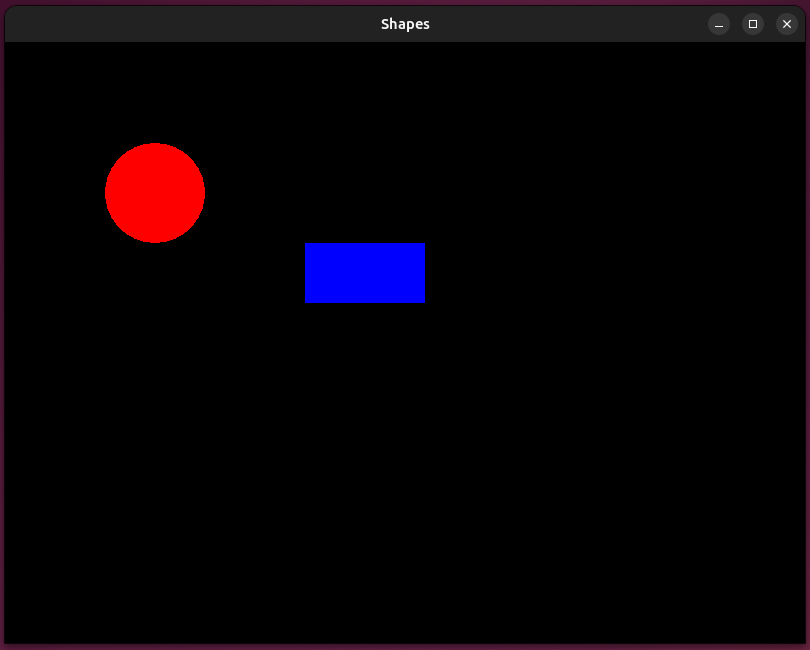
\includegraphics[width=0.8\textwidth]{src/img/sfml_shapes.png}
    \caption{Shapes}
    \label{fig:shapes}
\end{figure}

Рассмотрим обработку событий чуть подробнее. Пока запущено окно, оно постоянно проверяет было ли совершено какое-либо событие (нажатие клавиши, движение мыши и другие), если такое событие нашлось, то оно помещяется в очередь событий. Затем методом \texttt{pollEvent(event)} для окна мы вытаскиваем событие из очереди и присваиваем его переменной \texttt{event} класса \texttt{sf::Event}. После чего обрабатываем его и переходим к  следующему событию в случае, если очередь не пуста. Рассмотрим на примере движения мыши и нажатия клавиши \texttt{Escape}:

\begin{lstlisting}[style=myStyle]
if (event.type == sf::Event::KeyPressed) {
    if (event.key.code == sf::Keyboard::Escape)
        window.close();
}

if (event.type == sf::Event::MouseMoved) {
    std::cout << "Mouse position: " << event.mouseMove.x << ", " << event.mouseMove.y << std::endl;
}
\end{lstlisting}

Предварительно подключив заголовочный файл \texttt{iostream}, в результате получим, что при движении мыши в терминале будет обновляться её позиция, а по нажатию клавиши \texttt{Escape} программа завершится. Полный код (\autoref{lst:events}) и резульат (\autoref{fig:events}).
\begin{figure}[H]
    \centering
    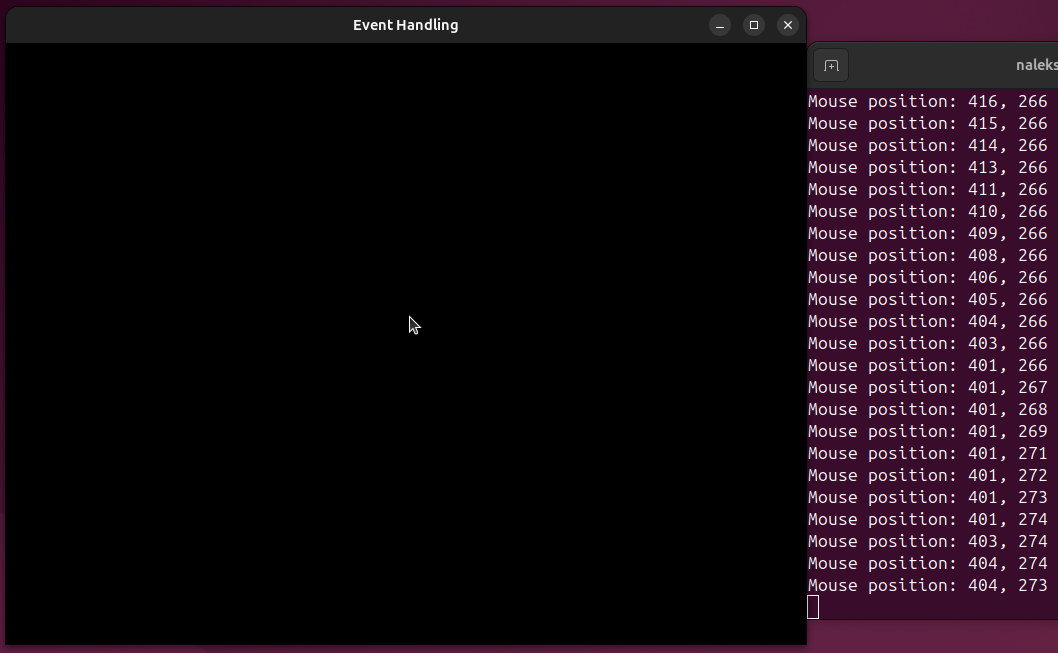
\includegraphics[width=0.8\textwidth]{src/img/sfml_events.png}
    \caption{Events}
    \label{fig:events}
\end{figure}

Последнее, что хотелось бы рассмотреть "--- это движение спрайта. В качестве последнего будет выступать круг, который мы уже умеем инициализировать и отображать. Реализуем самый простой способ движения "--- каждый кадр будем смещать спрайт на \texttt{X} и \texttt{Y} пикселей с помощью метода \texttt{move(X, Y)}. Для этого инициализируем нужные переменные и в основном цикле сдвинем спрайт:

\begin{lstlisting}[style=myStyle]
float speedX = 2.5f, speedY = 2.f;
ball.move(speedX, speedY);
\end{lstlisting}

Для того, чтобы постоянно в кадре наблюдать движение спрайта, пропишем простую логику. Пускай круг будет \flqq отскакивать\frqq\ от границ окна:

\begin{lstlisting}[style=myStyle]
if (ball.getPosition().x <= 0 || ball.getPosition().x >= 800 - 60) speedX = -speedX;
if (ball.getPosition().y <= 0 || ball.getPosition().y >= 600 - 60) speedY = -speedY;
\end{lstlisting}

Теперь мы можем постоянно наблюдать, как круг движется и \flqq ударяется\frqq\ о границы окна. На \autoref{fig:animation} светлым цветом показана текущая позиция круга, а на тёмных "--- позиции, которые он прошёл. В итоге движение получилось неидальным. Чтобы его улучшить (сделать более плавным) можно ограничить частоту кадров методом \texttt{setFramerateLimit()} для окна, а самый главный способ "--- преобразовать скорость из значения за кадр в значение, не зависящее от частоты кадров в секунду (\autoref{lst:animation}).
\begin{figure}[H]
    \centering
    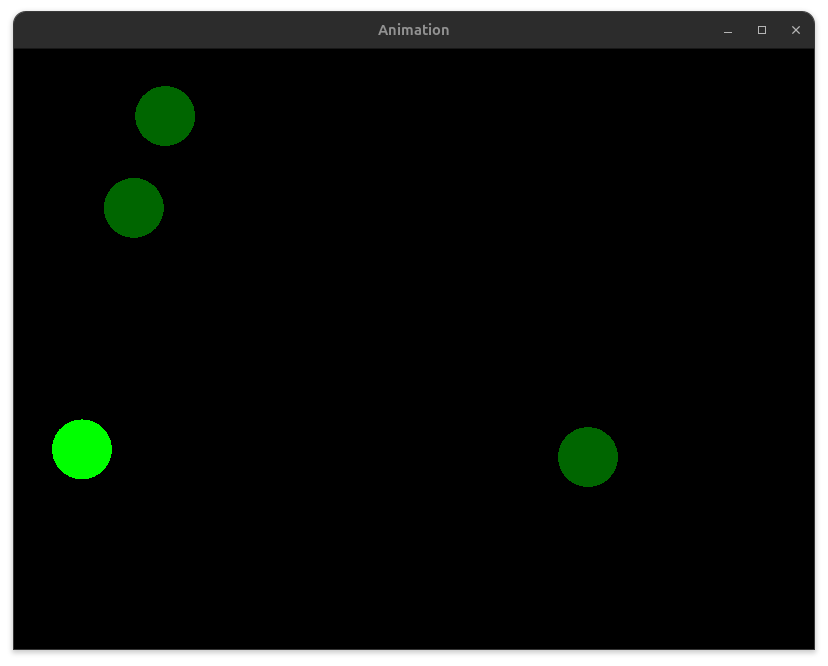
\includegraphics[width=0.8\textwidth]{src/img/sfml_animation.png}
    \caption{Animation}
    \label{fig:animation}
\end{figure}